% Options for packages loaded elsewhere
\PassOptionsToPackage{unicode}{hyperref}
\PassOptionsToPackage{hyphens}{url}
\PassOptionsToPackage{dvipsnames,svgnames,x11names}{xcolor}
%
\documentclass[
  letterpaper,
  DIV=11,
  numbers=noendperiod]{scrartcl}

\usepackage{amsmath,amssymb}
\usepackage{iftex}
\ifPDFTeX
  \usepackage[T1]{fontenc}
  \usepackage[utf8]{inputenc}
  \usepackage{textcomp} % provide euro and other symbols
\else % if luatex or xetex
  \usepackage{unicode-math}
  \defaultfontfeatures{Scale=MatchLowercase}
  \defaultfontfeatures[\rmfamily]{Ligatures=TeX,Scale=1}
\fi
\usepackage{lmodern}
\ifPDFTeX\else  
    % xetex/luatex font selection
\fi
% Use upquote if available, for straight quotes in verbatim environments
\IfFileExists{upquote.sty}{\usepackage{upquote}}{}
\IfFileExists{microtype.sty}{% use microtype if available
  \usepackage[]{microtype}
  \UseMicrotypeSet[protrusion]{basicmath} % disable protrusion for tt fonts
}{}
\makeatletter
\@ifundefined{KOMAClassName}{% if non-KOMA class
  \IfFileExists{parskip.sty}{%
    \usepackage{parskip}
  }{% else
    \setlength{\parindent}{0pt}
    \setlength{\parskip}{6pt plus 2pt minus 1pt}}
}{% if KOMA class
  \KOMAoptions{parskip=half}}
\makeatother
\usepackage{xcolor}
\setlength{\emergencystretch}{3em} % prevent overfull lines
\setcounter{secnumdepth}{-\maxdimen} % remove section numbering
% Make \paragraph and \subparagraph free-standing
\makeatletter
\ifx\paragraph\undefined\else
  \let\oldparagraph\paragraph
  \renewcommand{\paragraph}{
    \@ifstar
      \xxxParagraphStar
      \xxxParagraphNoStar
  }
  \newcommand{\xxxParagraphStar}[1]{\oldparagraph*{#1}\mbox{}}
  \newcommand{\xxxParagraphNoStar}[1]{\oldparagraph{#1}\mbox{}}
\fi
\ifx\subparagraph\undefined\else
  \let\oldsubparagraph\subparagraph
  \renewcommand{\subparagraph}{
    \@ifstar
      \xxxSubParagraphStar
      \xxxSubParagraphNoStar
  }
  \newcommand{\xxxSubParagraphStar}[1]{\oldsubparagraph*{#1}\mbox{}}
  \newcommand{\xxxSubParagraphNoStar}[1]{\oldsubparagraph{#1}\mbox{}}
\fi
\makeatother

\usepackage{color}
\usepackage{fancyvrb}
\newcommand{\VerbBar}{|}
\newcommand{\VERB}{\Verb[commandchars=\\\{\}]}
\DefineVerbatimEnvironment{Highlighting}{Verbatim}{commandchars=\\\{\}}
% Add ',fontsize=\small' for more characters per line
\usepackage{framed}
\definecolor{shadecolor}{RGB}{241,243,245}
\newenvironment{Shaded}{\begin{snugshade}}{\end{snugshade}}
\newcommand{\AlertTok}[1]{\textcolor[rgb]{0.68,0.00,0.00}{#1}}
\newcommand{\AnnotationTok}[1]{\textcolor[rgb]{0.37,0.37,0.37}{#1}}
\newcommand{\AttributeTok}[1]{\textcolor[rgb]{0.40,0.45,0.13}{#1}}
\newcommand{\BaseNTok}[1]{\textcolor[rgb]{0.68,0.00,0.00}{#1}}
\newcommand{\BuiltInTok}[1]{\textcolor[rgb]{0.00,0.23,0.31}{#1}}
\newcommand{\CharTok}[1]{\textcolor[rgb]{0.13,0.47,0.30}{#1}}
\newcommand{\CommentTok}[1]{\textcolor[rgb]{0.37,0.37,0.37}{#1}}
\newcommand{\CommentVarTok}[1]{\textcolor[rgb]{0.37,0.37,0.37}{\textit{#1}}}
\newcommand{\ConstantTok}[1]{\textcolor[rgb]{0.56,0.35,0.01}{#1}}
\newcommand{\ControlFlowTok}[1]{\textcolor[rgb]{0.00,0.23,0.31}{\textbf{#1}}}
\newcommand{\DataTypeTok}[1]{\textcolor[rgb]{0.68,0.00,0.00}{#1}}
\newcommand{\DecValTok}[1]{\textcolor[rgb]{0.68,0.00,0.00}{#1}}
\newcommand{\DocumentationTok}[1]{\textcolor[rgb]{0.37,0.37,0.37}{\textit{#1}}}
\newcommand{\ErrorTok}[1]{\textcolor[rgb]{0.68,0.00,0.00}{#1}}
\newcommand{\ExtensionTok}[1]{\textcolor[rgb]{0.00,0.23,0.31}{#1}}
\newcommand{\FloatTok}[1]{\textcolor[rgb]{0.68,0.00,0.00}{#1}}
\newcommand{\FunctionTok}[1]{\textcolor[rgb]{0.28,0.35,0.67}{#1}}
\newcommand{\ImportTok}[1]{\textcolor[rgb]{0.00,0.46,0.62}{#1}}
\newcommand{\InformationTok}[1]{\textcolor[rgb]{0.37,0.37,0.37}{#1}}
\newcommand{\KeywordTok}[1]{\textcolor[rgb]{0.00,0.23,0.31}{\textbf{#1}}}
\newcommand{\NormalTok}[1]{\textcolor[rgb]{0.00,0.23,0.31}{#1}}
\newcommand{\OperatorTok}[1]{\textcolor[rgb]{0.37,0.37,0.37}{#1}}
\newcommand{\OtherTok}[1]{\textcolor[rgb]{0.00,0.23,0.31}{#1}}
\newcommand{\PreprocessorTok}[1]{\textcolor[rgb]{0.68,0.00,0.00}{#1}}
\newcommand{\RegionMarkerTok}[1]{\textcolor[rgb]{0.00,0.23,0.31}{#1}}
\newcommand{\SpecialCharTok}[1]{\textcolor[rgb]{0.37,0.37,0.37}{#1}}
\newcommand{\SpecialStringTok}[1]{\textcolor[rgb]{0.13,0.47,0.30}{#1}}
\newcommand{\StringTok}[1]{\textcolor[rgb]{0.13,0.47,0.30}{#1}}
\newcommand{\VariableTok}[1]{\textcolor[rgb]{0.07,0.07,0.07}{#1}}
\newcommand{\VerbatimStringTok}[1]{\textcolor[rgb]{0.13,0.47,0.30}{#1}}
\newcommand{\WarningTok}[1]{\textcolor[rgb]{0.37,0.37,0.37}{\textit{#1}}}

\providecommand{\tightlist}{%
  \setlength{\itemsep}{0pt}\setlength{\parskip}{0pt}}\usepackage{longtable,booktabs,array}
\usepackage{calc} % for calculating minipage widths
% Correct order of tables after \paragraph or \subparagraph
\usepackage{etoolbox}
\makeatletter
\patchcmd\longtable{\par}{\if@noskipsec\mbox{}\fi\par}{}{}
\makeatother
% Allow footnotes in longtable head/foot
\IfFileExists{footnotehyper.sty}{\usepackage{footnotehyper}}{\usepackage{footnote}}
\makesavenoteenv{longtable}
\usepackage{graphicx}
\makeatletter
\def\maxwidth{\ifdim\Gin@nat@width>\linewidth\linewidth\else\Gin@nat@width\fi}
\def\maxheight{\ifdim\Gin@nat@height>\textheight\textheight\else\Gin@nat@height\fi}
\makeatother
% Scale images if necessary, so that they will not overflow the page
% margins by default, and it is still possible to overwrite the defaults
% using explicit options in \includegraphics[width, height, ...]{}
\setkeys{Gin}{width=\maxwidth,height=\maxheight,keepaspectratio}
% Set default figure placement to htbp
\makeatletter
\def\fps@figure{htbp}
\makeatother

\usepackage{fvextra}
\DefineVerbatimEnvironment{Highlighting}{Verbatim}{breaklines,commandchars=\\\{\}}
\DefineVerbatimEnvironment{OutputCode}{Verbatim}{breaklines,commandchars=\\\{\}}
\KOMAoption{captions}{tableheading}
\makeatletter
\@ifpackageloaded{caption}{}{\usepackage{caption}}
\AtBeginDocument{%
\ifdefined\contentsname
  \renewcommand*\contentsname{Table of contents}
\else
  \newcommand\contentsname{Table of contents}
\fi
\ifdefined\listfigurename
  \renewcommand*\listfigurename{List of Figures}
\else
  \newcommand\listfigurename{List of Figures}
\fi
\ifdefined\listtablename
  \renewcommand*\listtablename{List of Tables}
\else
  \newcommand\listtablename{List of Tables}
\fi
\ifdefined\figurename
  \renewcommand*\figurename{Figure}
\else
  \newcommand\figurename{Figure}
\fi
\ifdefined\tablename
  \renewcommand*\tablename{Table}
\else
  \newcommand\tablename{Table}
\fi
}
\@ifpackageloaded{float}{}{\usepackage{float}}
\floatstyle{ruled}
\@ifundefined{c@chapter}{\newfloat{codelisting}{h}{lop}}{\newfloat{codelisting}{h}{lop}[chapter]}
\floatname{codelisting}{Listing}
\newcommand*\listoflistings{\listof{codelisting}{List of Listings}}
\makeatother
\makeatletter
\makeatother
\makeatletter
\@ifpackageloaded{caption}{}{\usepackage{caption}}
\@ifpackageloaded{subcaption}{}{\usepackage{subcaption}}
\makeatother

\ifLuaTeX
  \usepackage{selnolig}  % disable illegal ligatures
\fi
\usepackage{bookmark}

\IfFileExists{xurl.sty}{\usepackage{xurl}}{} % add URL line breaks if available
\urlstyle{same} % disable monospaced font for URLs
\hypersetup{
  pdftitle={HW 1},
  pdfauthor={Bryan Mui - UID 506021334 - 14 April 2025},
  colorlinks=true,
  linkcolor={blue},
  filecolor={Maroon},
  citecolor={Blue},
  urlcolor={Blue},
  pdfcreator={LaTeX via pandoc}}


\title{HW 1}
\author{Bryan Mui - UID 506021334 - 14 April 2025}
\date{}

\begin{document}
\maketitle


Loaded packages: ggplot2, tidyverse (include = false for this chunk)

\section{Problem 1}\label{problem-1}

\subsection{Part a}\label{part-a}

Find the theoretical min for the function: \[
f(x) = x^4 + 2x^2 + 1
\]

Solution: find f'(x) and f'\,`(x), set f'(x) to 0 and solve, and
f'\,'(x) needs to be \textgreater{} 0 to be a min

Step 1: find f'(x) and f'\,'(x) \begin{align}
  f(x) &= x^4 + 2x^2 + 1 \\ 
 f'(x) &= 4x^3 + 4x  \\
f''(x) &= 12x^2 + 4 \\
\end {align}

Step 2: set f'(x) to 0 and solve

\begin{align}
f'(x) &= 4x^3 + 4x  \\
    0 &= 4x^3 + 4x \\
    0 &= 4x(x^2 + 4)
\end{align}

We get \[x = 0\] and \[0 = x^2 +4\] which has no real solution

Step 3: check that f'\,'(x) needs to be \textgreater{} 0 to be a min

Our critical point is x = 0,

\begin{align}
f''(0)  &= 12(0)^2 + 4 \\
        &= 4
\end{align}

Since f'(x) = 0 at 0 and f'\,'(x) \textgreater{} 0 at that point,
\textbf{we have a min at x = 0, and plugging into f(0) we get the
minimum point}

\begin{center} (0, 1) \end{center}

\subsection{Part b}\label{part-b}

\subsubsection{0)}\label{section}

Use the gradient descent algorithm with \textbf{constant step size} and
with \textbf{back-tracking line search} to calculate \(x_{min}\)

\textbf{Constant step size descent is implemented as follows:}

\begin{enumerate}
\def\labelenumi{\arabic{enumi}.}
\tightlist
\item
  Select a random starting point \(x_0\)\\
\item
  While stopping criteria \textless{} tolerance, do:
\end{enumerate}

\begin{itemize}
\tightlist
\item
  Select \(η_k\)(as a constant)\\
\item
  Calculate \(x_{(k+1)} = x_k - η_k * ∇(f(x_k))\)\\
\item
  Calculate the value of stopping criterion
\end{itemize}

Stopping criteria: Stop if \(∣|∇(f(x_k)||_2 ≤ ϵ\)

\begin{Shaded}
\begin{Highlighting}[]
\CommentTok{\# Gradient descent algorithm that uses backtracking to minimize an objective function}

\NormalTok{gradient\_descent\_constant\_step }\OtherTok{\textless{}{-}} \ControlFlowTok{function}\NormalTok{(}\AttributeTok{tol =} \FloatTok{1e{-}6}\NormalTok{, }\AttributeTok{max\_iter =} \DecValTok{10000}\NormalTok{, }\AttributeTok{step\_size =} \FloatTok{0.01}\NormalTok{) \{}
  \CommentTok{\# Step 1: Initialize and select a random stopping point}
  \CommentTok{\# Initialize}
  \FunctionTok{set.seed}\NormalTok{(}\DecValTok{777}\NormalTok{) }\CommentTok{\# example seeding }
\NormalTok{  last\_iter }\OtherTok{\textless{}{-}} \DecValTok{0} \CommentTok{\# the last iteration ran}
\NormalTok{  eta }\OtherTok{\textless{}{-}}\NormalTok{ step\_size }\CommentTok{\# step size that is decided manually }
\NormalTok{  max\_iter }\OtherTok{\textless{}{-}}\NormalTok{ max\_iter }\CommentTok{\# max iterations before terminating if mininum isn\textquotesingle{}t found}
\NormalTok{  tolerance }\OtherTok{\textless{}{-}}\NormalTok{ tol }\CommentTok{\# tolerance for the stoppign criteria }
\NormalTok{  obj\_values }\OtherTok{\textless{}{-}} \FunctionTok{numeric}\NormalTok{(max\_iter) }\CommentTok{\# Stores the value of f(x)}
\NormalTok{  eta\_values }\OtherTok{\textless{}{-}} \FunctionTok{numeric}\NormalTok{(max\_iter)  }\CommentTok{\# To store eta values used each iteration}
\NormalTok{  eta\_values[}\DecValTok{1}\NormalTok{] }\OtherTok{\textless{}{-}}\NormalTok{ step\_size}
\NormalTok{  betas }\OtherTok{\textless{}{-}} \FunctionTok{numeric}\NormalTok{(max\_iter) }\CommentTok{\# Stores the value of x guesses}
\NormalTok{  x0 }\OtherTok{\textless{}{-}} \FunctionTok{runif}\NormalTok{(}\DecValTok{1}\NormalTok{, }\AttributeTok{min=}\SpecialCharTok{{-}}\DecValTok{10}\NormalTok{, }\AttributeTok{max=}\DecValTok{10}\NormalTok{) }\CommentTok{\# our first guess is somewhere between {-}10{-}10}
  
  \CommentTok{\# Set the objective function to the function to be minimized }
  \CommentTok{\# Objective function: f(x)}
\NormalTok{  obj\_function }\OtherTok{\textless{}{-}} \ControlFlowTok{function}\NormalTok{(x) \{}
    \FunctionTok{return}\NormalTok{(x}\SpecialCharTok{\^{}}\DecValTok{4} \SpecialCharTok{+} \DecValTok{2}\SpecialCharTok{*}\NormalTok{(x}\SpecialCharTok{\^{}}\DecValTok{2}\NormalTok{) }\SpecialCharTok{+} \DecValTok{1}\NormalTok{) }
\NormalTok{  \}}
  
  \CommentTok{\# Gradient function: d/dx of f(x)}
\NormalTok{  gradient }\OtherTok{\textless{}{-}} \ControlFlowTok{function}\NormalTok{(x) \{}
    \FunctionTok{return}\NormalTok{(}\DecValTok{4}\SpecialCharTok{*}\NormalTok{x}\SpecialCharTok{\^{}}\DecValTok{3} \SpecialCharTok{+} \DecValTok{4}\SpecialCharTok{*}\NormalTok{x)}
\NormalTok{  \}}
  
  \CommentTok{\# Append the first guess to the obj\_values and betas vector}
\NormalTok{  betas[}\DecValTok{1}\NormalTok{] }\OtherTok{\textless{}{-}}\NormalTok{ x0}
\NormalTok{  obj\_values[}\DecValTok{1}\NormalTok{] }\OtherTok{\textless{}{-}} \FunctionTok{obj\_function}\NormalTok{(x0)}
  
  \CommentTok{\# Step 2: While stopping criteria \textless{} tolerance, do:}
  \ControlFlowTok{for}\NormalTok{ (iter }\ControlFlowTok{in} \DecValTok{1}\SpecialCharTok{:}\NormalTok{max\_iter) \{ }\CommentTok{\# the iteration goes n = 1, 2, 3, 4, but the arrays of our output starts at iter = 0 and guess x0}
    \CommentTok{\# Select eta(step size), which is constant}
    \CommentTok{\# There\textquotesingle{}s nothing to do for this step}
    
    \CommentTok{\# Calculate the next guess of x\_k+1, calculate f(x\_k+1), set eta(x\_k+1)}
\NormalTok{    betas[iter }\SpecialCharTok{+} \DecValTok{1}\NormalTok{] }\OtherTok{\textless{}{-}}\NormalTok{ betas[iter] }\SpecialCharTok{{-}}\NormalTok{ (eta }\SpecialCharTok{*} \FunctionTok{gradient}\NormalTok{(betas[iter]))}
\NormalTok{    obj\_values[iter }\SpecialCharTok{+} \DecValTok{1}\NormalTok{] }\OtherTok{\textless{}{-}} \FunctionTok{obj\_function}\NormalTok{(betas[iter }\SpecialCharTok{+} \DecValTok{1}\NormalTok{])}
\NormalTok{    eta\_values[iter }\SpecialCharTok{+} \DecValTok{1}\NormalTok{] }\OtherTok{\textless{}{-}}\NormalTok{ eta}
    
    \CommentTok{\# Calculate the value of the stopping criterion}
\NormalTok{    stop\_criteria }\OtherTok{\textless{}{-}} \FunctionTok{abs}\NormalTok{(}\FunctionTok{gradient}\NormalTok{(betas[iter }\SpecialCharTok{+} \DecValTok{1}\NormalTok{]))}
    
    \CommentTok{\# If stopping criteria less than tolerance, break}
    \ControlFlowTok{if}\NormalTok{(}\FunctionTok{is.na}\NormalTok{(stop\_criteria) }\SpecialCharTok{||}\NormalTok{ stop\_criteria }\SpecialCharTok{\textless{}=}\NormalTok{ tolerance) \{ }
\NormalTok{      last\_iter }\OtherTok{\textless{}{-}}\NormalTok{ iter }\SpecialCharTok{+} \DecValTok{1}
      \ControlFlowTok{break} 
\NormalTok{    \}}
    
    \CommentTok{\# if we never set last iter, then we hit the max number of iterations and need to set}
    \ControlFlowTok{if}\NormalTok{(last\_iter }\SpecialCharTok{==} \DecValTok{0}\NormalTok{) \{ last\_iter }\OtherTok{\textless{}{-}}\NormalTok{ max\_iter \}}
    
    \CommentTok{\# end algorithm}
\NormalTok{  \}}
  
  \FunctionTok{return}\NormalTok{(}\FunctionTok{list}\NormalTok{(}\AttributeTok{betas =}\NormalTok{ betas, }\AttributeTok{obj\_values =}\NormalTok{ obj\_values, }\AttributeTok{eta\_values =}\NormalTok{ eta\_values, }\AttributeTok{last\_iter =}\NormalTok{ last\_iter)) }\CommentTok{\# in this case, beta(predictors) are the x values, obj\_values are f(x), eta is the step size, last iter is the value in the vector of the final iteration before stopping}
\NormalTok{\}}
\end{Highlighting}
\end{Shaded}

Running the gradient descent algorithm with fixed step size:

\begin{Shaded}
\begin{Highlighting}[]
\NormalTok{minimize\_constant\_step }\OtherTok{\textless{}{-}} \FunctionTok{gradient\_descent\_constant\_step}\NormalTok{(}\AttributeTok{tol =} \FloatTok{1e{-}6}\NormalTok{, }\AttributeTok{max\_iter =} \DecValTok{10000}\NormalTok{, }\AttributeTok{step\_size =} \FloatTok{0.03}\NormalTok{)}
\FunctionTok{print}\NormalTok{(minimize\_constant\_step)}
\end{Highlighting}
\end{Shaded}

\begin{verbatim}
$betas
 [1]  3.757148134 -3.058091092  0.740763042  0.603094019  0.504399680
 [6]  0.428472253  0.367616075  0.317540520  0.275593469  0.240010435
[11]  0.209550087  0.183299884  0.160564858  0.140800331  0.123569332
[16]  0.108514593  0.095339505  0.083794772  0.073668795  0.064780563
[21]  0.056974273  0.050115167  0.044086243  0.038785612  0.034124337
[26]  0.030024648  0.026418442  0.023246017  0.020454987  0.017999362
[31]  0.015838739  0.013937613  0.012264775  0.010792780  0.009497496
[36]  0.008357693  0.007354700  0.006472088  0.005695405  0.005011934
[41]  0.004410487  0.003881218  0.003415465  0.003005605  0.002644929
[46]  0.002327535  0.002048229  0.001802441  0.001586147  0.001395809
 [ reached 'max' / getOption("max.print") -- omitted 9950 entries ]

$obj_values
 [1] 228.498357 107.162271   2.398564   1.859739   1.573567   1.400882
 [7]   1.288546   1.211831   1.157672   1.118528   1.089751   1.068327
[13]   1.052227   1.040042   1.030772   1.023689   1.018262   1.014092
[19]   1.010884   1.008411   1.006503   1.005029   1.003891   1.003011
[25]   1.002330   1.001804   1.001396   1.001081   1.000837   1.000648
[31]   1.000502   1.000389   1.000301   1.000233   1.000180   1.000140
[37]   1.000108   1.000084   1.000065   1.000050   1.000039   1.000030
[43]   1.000023   1.000018   1.000014   1.000011   1.000008   1.000006
[49]   1.000005   1.000004
 [ reached 'max' / getOption("max.print") -- omitted 9950 entries ]

$eta_values
 [1] 0.03 0.03 0.03 0.03 0.03 0.03 0.03 0.03 0.03 0.03 0.03 0.03 0.03 0.03 0.03
[16] 0.03 0.03 0.03 0.03 0.03 0.03 0.03 0.03 0.03 0.03 0.03 0.03 0.03 0.03 0.03
[31] 0.03 0.03 0.03 0.03 0.03 0.03 0.03 0.03 0.03 0.03 0.03 0.03 0.03 0.03 0.03
[46] 0.03 0.03 0.03 0.03 0.03
 [ reached 'max' / getOption("max.print") -- omitted 9950 entries ]

$last_iter
[1] 118
\end{verbatim}

\begin{Shaded}
\begin{Highlighting}[]
\FunctionTok{cat}\NormalTok{(}\StringTok{"The functions stopped after"}\NormalTok{, minimize\_constant\_step}\SpecialCharTok{$}\NormalTok{last\_iter }\SpecialCharTok{{-}} \DecValTok{1}\NormalTok{, }\StringTok{"iterations }\SpecialCharTok{\textbackslash{}n}\StringTok{"}\NormalTok{)}
\end{Highlighting}
\end{Shaded}

\begin{verbatim}
The functions stopped after 117 iterations 
\end{verbatim}

\begin{Shaded}
\begin{Highlighting}[]
\FunctionTok{cat}\NormalTok{(}\StringTok{"The function\textquotesingle{}s point of minimization is"}\NormalTok{, }\StringTok{"("}\NormalTok{, minimize\_constant\_step}\SpecialCharTok{$}\NormalTok{betas[minimize\_constant\_step}\SpecialCharTok{$}\NormalTok{last\_iter], }\StringTok{","}\NormalTok{ , minimize\_constant\_step}\SpecialCharTok{$}\NormalTok{obj\_values[minimize\_constant\_step}\SpecialCharTok{$}\NormalTok{last\_iter], }\StringTok{") }\SpecialCharTok{\textbackslash{}n}\StringTok{"}\NormalTok{)}
\end{Highlighting}
\end{Shaded}

\begin{verbatim}
The function's point of minimization is ( 2.342325e-07 , 1 ) 
\end{verbatim}

\textbf{Backtracking Line Search is implemented as follows:}

\begin{enumerate}
\def\labelenumi{\arabic{enumi}.}
\tightlist
\item
  Select a random starting point \(x_0\)\\
\item
  While stopping criteria \textless{} tolerance, do:
\end{enumerate}

\begin{itemize}
\tightlist
\item
  Select \(η_k\) using backtracking line search
\item
  Calculate \(x_{(k+1)} = x_k - η_k * ∇(f(x_k))\)\\
\item
  Calculate the value of stopping criterion
\end{itemize}

Backtracking Line Search:

\begin{itemize}
\tightlist
\item
  Set \(η^0 > 0\)(usually a large value), \(ϵ ∈ (0,1)\) and
  \(τ ∈ (0,1)\)
\item
  Set \(η_1 = η^0\)
\item
  At iteration k, set \(η_k <- η_{k-1}\)

  \begin{enumerate}
  \def\labelenumi{\arabic{enumi}.}
  \tightlist
  \item
    Check whether the Armijo Condition holds: \[
    h(η_k) ≤ h(0) + ϵη_kh'(0)
    \]\\
    where \(h(η_k) = f(x_k) − η_k ∇f(x_k)\)
  \item
  \end{enumerate}

  \begin{itemize}
  \tightlist
  \item
    If yes(condition holds), terminate and keep \(η_k\)
  \item
    If no, set \(η_k = τη_k\) and go to Step 1
  \end{itemize}
\end{itemize}

Stopping criteria: Stop if \(∣|∇(f(x_k)||_2 ≤ ϵ\)

Other note: Since we need h'(0) for the Armijo condition calculation,
that is given by:\\
\[
h'(0) = -[∇f(x_k)]^\top ∇f(x_k)
\] Since we are minimizing x, we have a one dimensional beta, we can
simplify to\\
\[
h'(0) = -||∇f(x_k)||^2
\]

To summarize, backtracking line search chooses the step size by ensuring
the Armijo condition always holds. If the Armijo condition doesn't hold,
we are probably overshooting, hence the step size gets updated
iteratively

\begin{Shaded}
\begin{Highlighting}[]
\NormalTok{gradient\_descent\_backtracking }\OtherTok{\textless{}{-}} \ControlFlowTok{function}\NormalTok{(}\AttributeTok{tol =} \FloatTok{1e{-}6}\NormalTok{, }\AttributeTok{max\_iter =} \DecValTok{10000}\NormalTok{, }\AttributeTok{epsilon =} \FloatTok{0.5}\NormalTok{, }\AttributeTok{tau =} \FloatTok{0.5}\NormalTok{, }\AttributeTok{init\_step\_size =} \DecValTok{1}\NormalTok{) \{}
  \CommentTok{\# Step 1: Initialize and select a random stopping point}
  \CommentTok{\# Initialize}
  \FunctionTok{set.seed}\NormalTok{(}\DecValTok{777}\NormalTok{) }\CommentTok{\# example seeding }
\NormalTok{  last\_iter }\OtherTok{\textless{}{-}} \DecValTok{0} \CommentTok{\# the last iteration ran}
\NormalTok{  max\_iter }\OtherTok{\textless{}{-}}\NormalTok{ max\_iter }\CommentTok{\# max iterations before terminating if minimum isn\textquotesingle{}t found}
\NormalTok{  tolerance }\OtherTok{\textless{}{-}}\NormalTok{ tol }\CommentTok{\# tolerance for the stopping criteria }
\NormalTok{  epsilon }\OtherTok{\textless{}{-}}\NormalTok{ epsilon }\CommentTok{\# Epsilon used in the step size criteria calculation}
\NormalTok{  tau }\OtherTok{\textless{}{-}}\NormalTok{ tau }\CommentTok{\# tau used in the step size criteria calculation}
\NormalTok{  obj\_values }\OtherTok{\textless{}{-}} \FunctionTok{numeric}\NormalTok{(max\_iter) }\CommentTok{\# Stores the value of f(x)}
\NormalTok{  eta\_values }\OtherTok{\textless{}{-}} \FunctionTok{numeric}\NormalTok{(max\_iter)  }\CommentTok{\# To store eta values used each iteration}
\NormalTok{  eta\_values[}\DecValTok{1}\NormalTok{] }\OtherTok{\textless{}{-}}\NormalTok{ init\_step\_size}
\NormalTok{  betas }\OtherTok{\textless{}{-}} \FunctionTok{numeric}\NormalTok{(max\_iter) }\CommentTok{\# Stores the value of x guesses}
\NormalTok{  x0 }\OtherTok{\textless{}{-}} \FunctionTok{runif}\NormalTok{(}\DecValTok{1}\NormalTok{, }\AttributeTok{min=}\SpecialCharTok{{-}}\DecValTok{10}\NormalTok{, }\AttributeTok{max=}\DecValTok{10}\NormalTok{) }\CommentTok{\# our first guess is somewhere between {-}10 to 10}
\NormalTok{  eta }\OtherTok{\textless{}{-}}\NormalTok{ init\_step\_size }\CommentTok{\# our initial step size}
  
  \CommentTok{\# Set the objective function to the function to be minimized }
  \CommentTok{\# Objective function: f(x)}
\NormalTok{  obj\_function }\OtherTok{\textless{}{-}} \ControlFlowTok{function}\NormalTok{(x) \{}
    \FunctionTok{return}\NormalTok{(x}\SpecialCharTok{\^{}}\DecValTok{4} \SpecialCharTok{+} \DecValTok{2}\SpecialCharTok{*}\NormalTok{(x}\SpecialCharTok{\^{}}\DecValTok{2}\NormalTok{) }\SpecialCharTok{+} \DecValTok{1}\NormalTok{) }
\NormalTok{  \}}
  
  \CommentTok{\# Gradient function: d/dx of f(x)}
\NormalTok{  gradient }\OtherTok{\textless{}{-}} \ControlFlowTok{function}\NormalTok{(x) \{}
    \FunctionTok{return}\NormalTok{(}\DecValTok{4}\SpecialCharTok{*}\NormalTok{x}\SpecialCharTok{\^{}}\DecValTok{3} \SpecialCharTok{+} \DecValTok{4}\SpecialCharTok{*}\NormalTok{x)}
\NormalTok{  \}}
  
  \CommentTok{\# Armijo condition function}
  \CommentTok{\# returns TRUE or FALSE whether the condition is satisfied or not}
\NormalTok{  armijo\_stepsize }\OtherTok{\textless{}{-}} \ControlFlowTok{function}\NormalTok{(beta, eta, grad, f, epsilon, tau, max\_iter) \{}
\NormalTok{    subiter }\OtherTok{\textless{}{-}} \DecValTok{1} \CommentTok{\# set a hard limit of iterations}
    \CommentTok{\# calc armijo}
\NormalTok{    beta\_new }\OtherTok{\textless{}{-}}\NormalTok{ beta }\SpecialCharTok{{-}}\NormalTok{ (eta)}\SpecialCharTok{*}\FunctionTok{grad}\NormalTok{(beta)}
\NormalTok{    armijo }\OtherTok{\textless{}{-}} \FunctionTok{f}\NormalTok{(beta\_new) }\SpecialCharTok{\textgreater{}}\NormalTok{ (}\FunctionTok{f}\NormalTok{(beta) }\SpecialCharTok{{-}}\NormalTok{ epsilon}\SpecialCharTok{*}\NormalTok{eta}\SpecialCharTok{*}\FunctionTok{sum}\NormalTok{(}\FunctionTok{grad}\NormalTok{(beta)}\SpecialCharTok{\^{}}\DecValTok{2}\NormalTok{))}
    \ControlFlowTok{while}\NormalTok{ (armijo }\SpecialCharTok{\&\&}\NormalTok{ (iter }\SpecialCharTok{\textless{}=}\NormalTok{ max\_iter)) \{}
      \CommentTok{\#update eta}
\NormalTok{      eta }\OtherTok{\textless{}{-}}\NormalTok{ tau }\SpecialCharTok{*}\NormalTok{ eta}
      
      \CommentTok{\#recalculate armijo}
\NormalTok{      beta\_new }\OtherTok{\textless{}{-}}\NormalTok{ beta }\SpecialCharTok{{-}}\NormalTok{ (eta)}\SpecialCharTok{*}\FunctionTok{grad}\NormalTok{(beta)}
\NormalTok{      armijo }\OtherTok{\textless{}{-}} \FunctionTok{f}\NormalTok{(beta\_new) }\SpecialCharTok{\textgreater{}}\NormalTok{ (}\FunctionTok{f}\NormalTok{(beta) }\SpecialCharTok{{-}}\NormalTok{ epsilon}\SpecialCharTok{*}\NormalTok{eta}\SpecialCharTok{*}\FunctionTok{sum}\NormalTok{(}\FunctionTok{grad}\NormalTok{(beta)}\SpecialCharTok{\^{}}\DecValTok{2}\NormalTok{))}
      
\NormalTok{      subiter }\OtherTok{\textless{}{-}}\NormalTok{ subiter }\SpecialCharTok{+} \DecValTok{1}
\NormalTok{    \}}
    \FunctionTok{return}\NormalTok{(eta)}
\NormalTok{  \}}
  
  \CommentTok{\# Append the first guess to the obj\_values and betas vector}
\NormalTok{  betas[}\DecValTok{1}\NormalTok{] }\OtherTok{\textless{}{-}}\NormalTok{ x0}
\NormalTok{  obj\_values[}\DecValTok{1}\NormalTok{] }\OtherTok{\textless{}{-}} \FunctionTok{obj\_function}\NormalTok{(x0)}
  
  \CommentTok{\# Step 2: While stopping criteria \textless{} tolerance, do:}
  \ControlFlowTok{for}\NormalTok{ (iter }\ControlFlowTok{in} \DecValTok{1}\SpecialCharTok{:}\NormalTok{max\_iter) \{ }\CommentTok{\# the iteration goes n = 1, 2, 3, 4, but the arrays of our output starts at iter = 0 and guess x0}
\NormalTok{    beta }\OtherTok{\textless{}{-}}\NormalTok{ betas[iter]}
    
    \CommentTok{\# use BLS to calculate eta}
\NormalTok{    eta }\OtherTok{\textless{}{-}} \FunctionTok{armijo\_stepsize}\NormalTok{(}\AttributeTok{beta =}\NormalTok{ beta, }\AttributeTok{eta =}\NormalTok{ eta, }\AttributeTok{grad =}\NormalTok{ gradient, }\AttributeTok{f =}\NormalTok{ obj\_function, }\AttributeTok{epsilon =}\NormalTok{ epsilon, }\AttributeTok{tau =}\NormalTok{ tau, }\AttributeTok{max\_iter =}\NormalTok{ max\_iter)}
\NormalTok{    eta\_values[iter }\SpecialCharTok{+} \DecValTok{1}\NormalTok{] }\OtherTok{\textless{}{-}}\NormalTok{ eta}
    
    \CommentTok{\# Calculate the next guess of x\_k+1}
\NormalTok{    beta\_new }\OtherTok{\textless{}{-}}\NormalTok{ beta }\SpecialCharTok{{-}}\NormalTok{ (eta }\SpecialCharTok{*} \FunctionTok{gradient}\NormalTok{(beta))}
\NormalTok{    betas[iter }\SpecialCharTok{+} \DecValTok{1}\NormalTok{] }\OtherTok{\textless{}{-}}\NormalTok{ beta\_new}
    
    \CommentTok{\# calculate f(x\_k+1), to keep track obj values}
\NormalTok{    obj\_values[iter }\SpecialCharTok{+} \DecValTok{1}\NormalTok{] }\OtherTok{\textless{}{-}} \FunctionTok{obj\_function}\NormalTok{(beta\_new)}
    
    \CommentTok{\# Calculate the value of the stopping criterion}
\NormalTok{    stop\_criteria }\OtherTok{\textless{}{-}} \FunctionTok{abs}\NormalTok{(}\FunctionTok{gradient}\NormalTok{(beta\_new))}
    
    \CommentTok{\# If stopping criteria less than tolerance, break}
    \ControlFlowTok{if}\NormalTok{(}\FunctionTok{is.na}\NormalTok{(stop\_criteria) }\SpecialCharTok{||}\NormalTok{ stop\_criteria }\SpecialCharTok{\textless{}=}\NormalTok{ tolerance) \{ }
\NormalTok{      last\_iter }\OtherTok{\textless{}{-}}\NormalTok{ iter }\SpecialCharTok{+} \DecValTok{1}
      \ControlFlowTok{break} 
\NormalTok{    \}}
    
    \CommentTok{\# if we never set last iter, then we hit the max number of iterations and need to set}
    \ControlFlowTok{if}\NormalTok{(last\_iter }\SpecialCharTok{==} \DecValTok{0}\NormalTok{) \{ last\_iter }\OtherTok{\textless{}{-}}\NormalTok{ max\_iter \}}
    
    \CommentTok{\# end algorithm}
\NormalTok{  \}}
  
  \FunctionTok{return}\NormalTok{(}\FunctionTok{list}\NormalTok{(}\AttributeTok{betas =}\NormalTok{ betas, }\AttributeTok{obj\_values =}\NormalTok{ obj\_values, }\AttributeTok{eta\_values =}\NormalTok{ eta\_values, }\AttributeTok{last\_iter =}\NormalTok{ last\_iter)) }\CommentTok{\# in this case, beta(predictors) are the x values, obj\_values are f(x), eta is the step size, last iter is the value in the vector of the final iteration before stopping}
\NormalTok{\}}
\end{Highlighting}
\end{Shaded}

Running the gradient descent algorithm with backtracking:

\begin{Shaded}
\begin{Highlighting}[]
\NormalTok{minimize\_backtrack }\OtherTok{\textless{}{-}} \FunctionTok{gradient\_descent\_backtracking}\NormalTok{(}\AttributeTok{tol =} \FloatTok{1e{-}6}\NormalTok{, }\AttributeTok{max\_iter =} \DecValTok{10000}\NormalTok{, }\AttributeTok{epsilon =} \FloatTok{0.5}\NormalTok{, }\AttributeTok{tau =} \FloatTok{0.8}\NormalTok{, }\AttributeTok{init\_step\_size =} \DecValTok{1}\NormalTok{)}
\FunctionTok{print}\NormalTok{(minimize\_backtrack)}
\end{Highlighting}
\end{Shaded}

\begin{verbatim}
$betas
 [1] 3.7571481 2.0808951 1.7535339 1.5426377 1.3887564 1.2687146 1.1709946
 [8] 1.0890410 1.0187765 0.9574987 0.9033291 0.8549116 0.8112373 0.7715364
[15] 0.7352094 0.7017805 0.6708666 0.6421547 0.6153861 0.5903448 0.5668485
[22] 0.5447423 0.5238933 0.5041868 0.4855230 0.4678148 0.4509856 0.4349676
[29] 0.4197007 0.4051313 0.3912114 0.3778977 0.3651513 0.3529370 0.3412225
[36] 0.3299788 0.3191791 0.3087989 0.2988156 0.2892087 0.2799588 0.2710482
[43] 0.2624606 0.2541805 0.2461937 0.2384869 0.2310477 0.2238643 0.2169259
[50] 0.2102221
 [ reached 'max' / getOption("max.print") -- omitted 9950 entries ]

$obj_values
 [1] 228.498357  28.410229  16.604656  11.422582   8.576958   6.810204
 [7]   5.622724   4.778641   4.153059   3.674137   3.297869   2.995924
[13]   2.749315   2.544881   2.373241   2.227544   2.102680   1.994768
[19]   1.900814   1.818471   1.745879   1.681546   1.624259   1.573028
[25]   1.527035   1.485597   1.448143   1.414189   1.383326   1.355202
[31]   1.329516   1.306007   1.284449   1.264645   1.246422   1.229628
[37]   1.214129   1.199806   1.186554   1.174279   1.162897   1.152332
[43]   1.142516   1.133390   1.124896   1.116987   1.109616   1.102742
[49]   1.096328   1.090340
 [ reached 'max' / getOption("max.print") -- omitted 9950 entries ]

$eta_values
 [1] 1.000000000 0.007378698 0.007378698 0.007378698 0.007378698 0.007378698
 [7] 0.007378698 0.007378698 0.007378698 0.007378698 0.007378698 0.007378698
[13] 0.007378698 0.007378698 0.007378698 0.007378698 0.007378698 0.007378698
[19] 0.007378698 0.007378698 0.007378698 0.007378698 0.007378698 0.007378698
[25] 0.007378698 0.007378698 0.007378698 0.007378698 0.007378698 0.007378698
[31] 0.007378698 0.007378698 0.007378698 0.007378698 0.007378698 0.007378698
[37] 0.007378698 0.007378698 0.007378698 0.007378698 0.007378698 0.007378698
[43] 0.007378698 0.007378698 0.007378698 0.007378698 0.007378698 0.007378698
[49] 0.007378698 0.007378698
 [ reached 'max' / getOption("max.print") -- omitted 9950 entries ]

$last_iter
[1] 505
\end{verbatim}

\begin{Shaded}
\begin{Highlighting}[]
\FunctionTok{cat}\NormalTok{(}\StringTok{"The functions stopped after"}\NormalTok{, minimize\_backtrack}\SpecialCharTok{$}\NormalTok{last\_iter }\SpecialCharTok{{-}} \DecValTok{1}\NormalTok{, }\StringTok{"iterations }\SpecialCharTok{\textbackslash{}n}\StringTok{"}\NormalTok{)}
\end{Highlighting}
\end{Shaded}

\begin{verbatim}
The functions stopped after 504 iterations 
\end{verbatim}

\begin{Shaded}
\begin{Highlighting}[]
\FunctionTok{cat}\NormalTok{(}\StringTok{"The function\textquotesingle{}s point of minimization is"}\NormalTok{, }\StringTok{"("}\NormalTok{, minimize\_backtrack}\SpecialCharTok{$}\NormalTok{betas[minimize\_backtrack}\SpecialCharTok{$}\NormalTok{last\_iter], }\StringTok{","}\NormalTok{ , minimize\_backtrack}\SpecialCharTok{$}\NormalTok{obj\_values[minimize\_backtrack}\SpecialCharTok{$}\NormalTok{last\_iter], }\StringTok{") }\SpecialCharTok{\textbackslash{}n}\StringTok{"}\NormalTok{)}
\end{Highlighting}
\end{Shaded}

\begin{verbatim}
The function's point of minimization is ( 2.470678e-07 , 1 ) 
\end{verbatim}

\subsubsection{1) For the constant step size version of gradient
descent, discuss how you selected the step size used in your
code}\label{for-the-constant-step-size-version-of-gradient-descent-discuss-how-you-selected-the-step-size-used-in-your-code}

Theoretical Analysis proves that for functions with a unique global
minimum, the step size should be within 0 to 1/L to converge to the
unique global minimum, where L is the Lipchitz constant, given by:

\[
||∇f(x) - ∇f(y)||_2 \le L||x - y||_2
\] Since this cannot be calculated in practice, usually a small step
size of 0.01 is what to begin with. From there, manually fine tuning to
try 0.02 and 0.03 is a good idea to see if there's any better
iterations. Starting from a big step size is usually unsafe do the
algorithm overshooting and diverging instead of converging. Ultimately,
the step size of 0.02 seemed best to reduce the number of iterations.

\subsubsection{\texorpdfstring{2) For both versions of the gradient
descent algorithm, plot the value of \(f(x_k)\) as a function of k the
number of
iterations}{2) For both versions of the gradient descent algorithm, plot the value of f(x\_k) as a function of k the number of iterations}}\label{for-both-versions-of-the-gradient-descent-algorithm-plot-the-value-of-fx_k-as-a-function-of-k-the-number-of-iterations}

\begin{Shaded}
\begin{Highlighting}[]
\CommentTok{\# constant step size}
\NormalTok{iterations }\OtherTok{\textless{}{-}} \DecValTok{1}\SpecialCharTok{:}\NormalTok{minimize\_constant\_step}\SpecialCharTok{$}\NormalTok{last\_iter}
\NormalTok{obj\_values }\OtherTok{\textless{}{-}}\NormalTok{ (minimize\_constant\_step}\SpecialCharTok{$}\NormalTok{obj\_values)[iterations]}
\NormalTok{f\_k\_constant }\OtherTok{\textless{}{-}} \FunctionTok{cbind}\NormalTok{(obj\_values, iterations)}

\NormalTok{iterations }\OtherTok{\textless{}{-}} \DecValTok{1}\SpecialCharTok{:}\NormalTok{minimize\_backtrack}\SpecialCharTok{$}\NormalTok{last\_iter}
\NormalTok{obj\_values }\OtherTok{\textless{}{-}}\NormalTok{ (minimize\_backtrack}\SpecialCharTok{$}\NormalTok{obj\_values)[iterations]}
\NormalTok{f\_k\_backtrack }\OtherTok{\textless{}{-}} \FunctionTok{cbind}\NormalTok{(obj\_values, iterations)}

\FunctionTok{ggplot}\NormalTok{(f\_k\_constant, }\FunctionTok{aes}\NormalTok{(}\AttributeTok{x=}\NormalTok{iterations, }\AttributeTok{y=}\NormalTok{obj\_values)) }\SpecialCharTok{+} 
  \FunctionTok{geom\_point}\NormalTok{() }\SpecialCharTok{+} 
  \FunctionTok{geom\_line}\NormalTok{() }\SpecialCharTok{+} 
  \FunctionTok{ggtitle}\NormalTok{(}\StringTok{"Gradient Descent Convergence, Constant Step Size"}\NormalTok{) }\SpecialCharTok{+} 
  \FunctionTok{xlab}\NormalTok{(}\StringTok{"Iteration"}\NormalTok{) }\SpecialCharTok{+} \FunctionTok{ylab}\NormalTok{(}\StringTok{"Objective Function Value"}\NormalTok{)}
\end{Highlighting}
\end{Shaded}

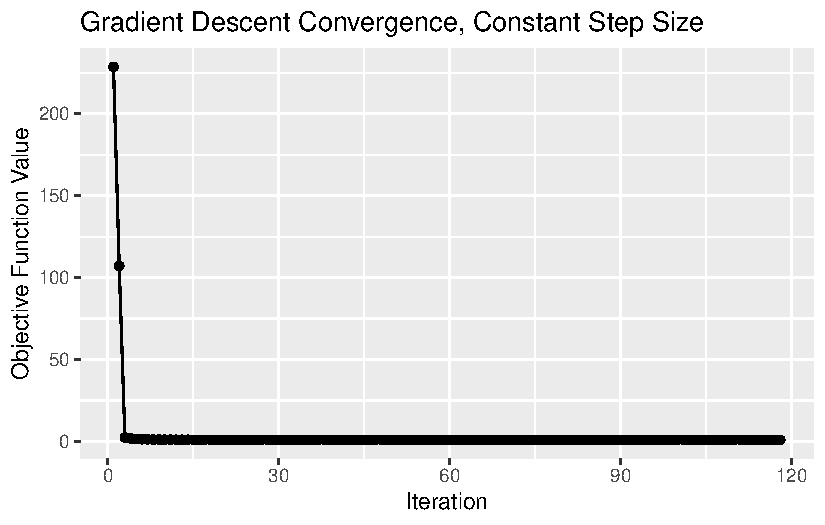
\includegraphics{506021334_Stats102B_hw_1_files/figure-pdf/unnamed-chunk-1-1.pdf}

\begin{Shaded}
\begin{Highlighting}[]
\FunctionTok{ggplot}\NormalTok{(f\_k\_backtrack, }\FunctionTok{aes}\NormalTok{(}\AttributeTok{x=}\NormalTok{iterations, }\AttributeTok{y=}\NormalTok{obj\_values)) }\SpecialCharTok{+} 
  \FunctionTok{geom\_point}\NormalTok{() }\SpecialCharTok{+} 
  \FunctionTok{geom\_line}\NormalTok{() }\SpecialCharTok{+} 
  \FunctionTok{ggtitle}\NormalTok{(}\StringTok{"Gradient Descent Convergence, Backtracking Line Search"}\NormalTok{) }\SpecialCharTok{+} 
  \FunctionTok{xlab}\NormalTok{(}\StringTok{"Iteration"}\NormalTok{) }\SpecialCharTok{+} \FunctionTok{ylab}\NormalTok{(}\StringTok{"Objective Function Value"}\NormalTok{)}
\end{Highlighting}
\end{Shaded}

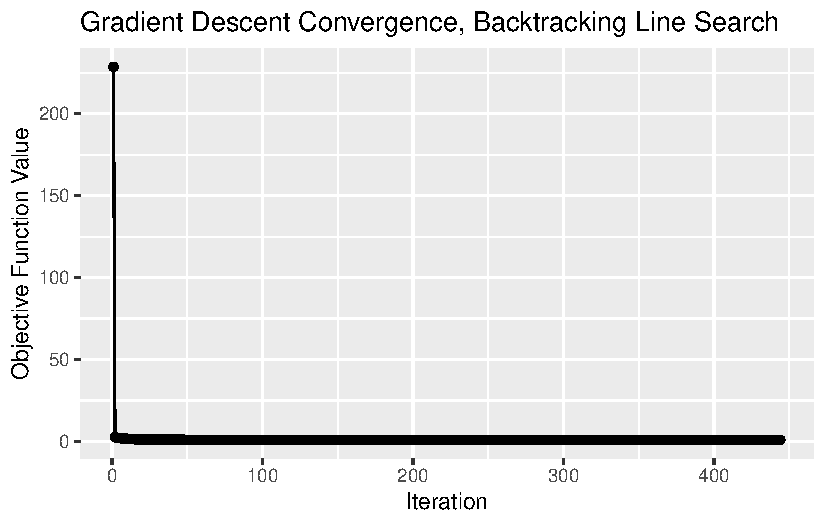
\includegraphics{506021334_Stats102B_hw_1_files/figure-pdf/unnamed-chunk-1-2.pdf}

\subsubsection{\texorpdfstring{3) For the the gradient descent method
with backtracking line search, plot the step size \(η_k\) selected at
step k as a function of k. Comment on the
result}{3) For the the gradient descent method with backtracking line search, plot the step size η\_k selected at step k as a function of k. Comment on the result}}\label{for-the-the-gradient-descent-method-with-backtracking-line-search-plot-the-step-size-ux3b7_k-selected-at-step-k-as-a-function-of-k.-comment-on-the-result}

\begin{Shaded}
\begin{Highlighting}[]
\NormalTok{iterations }\OtherTok{\textless{}{-}} \DecValTok{1}\SpecialCharTok{:}\NormalTok{minimize\_backtrack}\SpecialCharTok{$}\NormalTok{last\_iter}
\NormalTok{eta\_values }\OtherTok{\textless{}{-}}\NormalTok{ minimize\_backtrack}\SpecialCharTok{$}\NormalTok{eta\_values[iterations]}
\NormalTok{eta\_backtrack }\OtherTok{\textless{}{-}} \FunctionTok{cbind}\NormalTok{(eta\_values, iterations)}

\FunctionTok{ggplot}\NormalTok{(eta\_backtrack, }\FunctionTok{aes}\NormalTok{(}\AttributeTok{x=}\NormalTok{iterations, }\AttributeTok{y=}\NormalTok{eta\_values)) }\SpecialCharTok{+} 
  \FunctionTok{geom\_point}\NormalTok{(}\AttributeTok{color =} \StringTok{"blue"}\NormalTok{) }\SpecialCharTok{+} 
  \FunctionTok{geom\_line}\NormalTok{(}\AttributeTok{color =} \StringTok{"blue"}\NormalTok{) }\SpecialCharTok{+} 
  \FunctionTok{ggtitle}\NormalTok{(}\StringTok{"Gradient Descent Eta Values, BLS"}\NormalTok{) }\SpecialCharTok{+} 
  \FunctionTok{xlab}\NormalTok{(}\StringTok{"Iteration"}\NormalTok{) }\SpecialCharTok{+} \FunctionTok{ylab}\NormalTok{(}\StringTok{"Eta Value"}\NormalTok{)}
\end{Highlighting}
\end{Shaded}

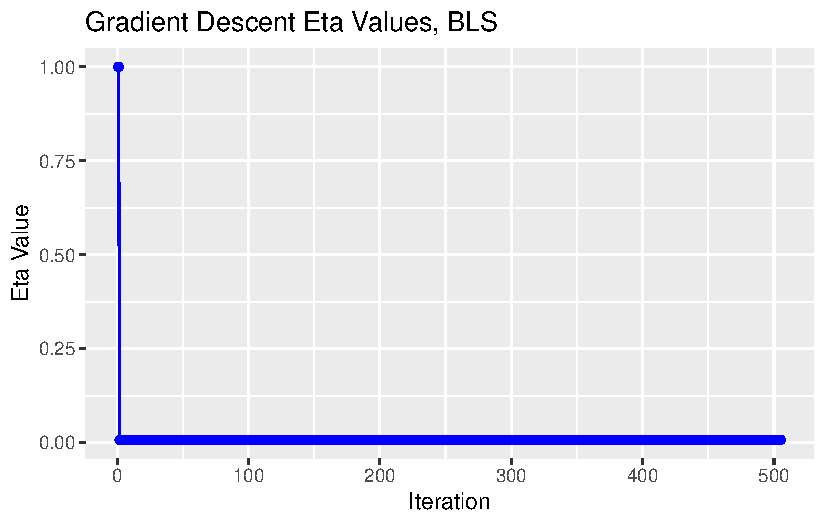
\includegraphics{506021334_Stats102B_hw_1_files/figure-pdf/unnamed-chunk-2-1.pdf}

We can see that the step size was initially 0.02, but at the very first
few iterations the Armijo condition immediately reduced the step size to
a very small number \textless{} 0.005 in order to prevent overshooting.
This condition held for the rest of the iterations until the algorithm
converged eventually, after around 443 iterations. Compared to the
constant step size gradient descent, the step size was much smaller for
all the iterations, meaning that it converged with \textgreater{} 300
more iterations than the constant step size gradient descent. Although
using a large step size like 0.02 would be much faster, it seems like
the step sizes were chosen to be a safer bound so that the algorithm
would not overshoot

\section{Problem 2}\label{problem-2}

\textbf{To understand the sensitivity of the gradient descent algorithm
and its variants to the ``shape'' of the function, the two data sets
provided (dataset1.csv, dataset2.csv) will be used}

They contain 100 observations for a response \(y\) and 20 predictors
\(x_j, j = 1, · · · , 20\)

\subsection{Part a}\label{part-a-1}

Using the gradient descent code provided (both in R and Python) obtain
the estimates of the regression coefficient, using both a constant step
size and backtracking line search.

Read in the data and the gradient descent function:

\begin{Shaded}
\begin{Highlighting}[]
\NormalTok{dataset1 }\OtherTok{\textless{}{-}} \FunctionTok{read\_csv}\NormalTok{(}\StringTok{"dataset1.csv"}\NormalTok{)}
\end{Highlighting}
\end{Shaded}

\begin{verbatim}
Rows: 100 Columns: 21
-- Column specification --------------------------------------------------------
Delimiter: ","
dbl (21): Y, X1, X2, X3, X4, X5, X6, X7, X8, X9, X10, X11, X12, X13, X14, X1...

i Use `spec()` to retrieve the full column specification for this data.
i Specify the column types or set `show_col_types = FALSE` to quiet this message.
\end{verbatim}

\begin{Shaded}
\begin{Highlighting}[]
\NormalTok{dataset2 }\OtherTok{\textless{}{-}} \FunctionTok{read\_csv}\NormalTok{(}\StringTok{"dataset2.csv"}\NormalTok{)}
\end{Highlighting}
\end{Shaded}

\begin{verbatim}
Rows: 100 Columns: 21
-- Column specification --------------------------------------------------------
Delimiter: ","
dbl (21): Y, X1, X2, X3, X4, X5, X6, X7, X8, X9, X10, X11, X12, X13, X14, X1...

i Use `spec()` to retrieve the full column specification for this data.
i Specify the column types or set `show_col_types = FALSE` to quiet this message.
\end{verbatim}

\begin{Shaded}
\begin{Highlighting}[]
\CommentTok{\# gradient descent given in class}
\NormalTok{gradient\_descent\_class }\OtherTok{\textless{}{-}} \ControlFlowTok{function}\NormalTok{(X, y, }\AttributeTok{eta =} \ConstantTok{NULL}\NormalTok{, }\AttributeTok{tol =} \FloatTok{1e{-}6}\NormalTok{, }\AttributeTok{max\_iter =} \DecValTok{10000}\NormalTok{, }\AttributeTok{backtracking =} \ConstantTok{TRUE}\NormalTok{, }\AttributeTok{epsilon =} \FloatTok{0.5}\NormalTok{, }\AttributeTok{tau =} \FloatTok{0.8}\NormalTok{) \{}
  \CommentTok{\# Initialize}
\NormalTok{  n }\OtherTok{\textless{}{-}} \FunctionTok{nrow}\NormalTok{(X)}
\NormalTok{  p }\OtherTok{\textless{}{-}} \FunctionTok{ncol}\NormalTok{(X)}
\NormalTok{  beta }\OtherTok{\textless{}{-}} \FunctionTok{rep}\NormalTok{(}\DecValTok{0}\NormalTok{, p)}
\NormalTok{  obj\_values }\OtherTok{\textless{}{-}} \FunctionTok{numeric}\NormalTok{(max\_iter)}
\NormalTok{  eta\_values }\OtherTok{\textless{}{-}} \FunctionTok{numeric}\NormalTok{(max\_iter)  }\CommentTok{\# To store eta values used each iteration}
\NormalTok{  eta\_bt }\OtherTok{\textless{}{-}} \DecValTok{1}  \CommentTok{\# Initial step size for backtracking}
  
  \CommentTok{\# Objective function: Mean Squared Error (MSE)}
\NormalTok{  obj\_function }\OtherTok{\textless{}{-}} \ControlFlowTok{function}\NormalTok{(beta) \{}
    \FunctionTok{sum}\NormalTok{((X }\SpecialCharTok{\%*\%}\NormalTok{ beta }\SpecialCharTok{{-}}\NormalTok{ y)}\SpecialCharTok{\^{}}\DecValTok{2}\NormalTok{) }\SpecialCharTok{/}\NormalTok{ (}\DecValTok{2} \SpecialCharTok{*}\NormalTok{ n)}
\NormalTok{  \}}
  
  \CommentTok{\# Gradient function}
\NormalTok{  gradient }\OtherTok{\textless{}{-}} \ControlFlowTok{function}\NormalTok{(beta) \{}
    \FunctionTok{t}\NormalTok{(X) }\SpecialCharTok{\%*\%}\NormalTok{ (X }\SpecialCharTok{\%*\%}\NormalTok{ beta }\SpecialCharTok{{-}}\NormalTok{ y) }\SpecialCharTok{/}\NormalTok{ n}
\NormalTok{  \}}
  
  \ControlFlowTok{for}\NormalTok{ (iter }\ControlFlowTok{in} \DecValTok{1}\SpecialCharTok{:}\NormalTok{max\_iter) \{}
\NormalTok{    grad }\OtherTok{\textless{}{-}} \FunctionTok{gradient}\NormalTok{(beta)}
    
    \ControlFlowTok{if}\NormalTok{ (backtracking) \{}
      \ControlFlowTok{if}\NormalTok{ (iter }\SpecialCharTok{==} \DecValTok{1}\NormalTok{) eta\_bt }\OtherTok{\textless{}{-}} \DecValTok{1}  \CommentTok{\# Reset only in the first iteration}
\NormalTok{      beta\_new }\OtherTok{\textless{}{-}}\NormalTok{ beta }\SpecialCharTok{{-}}\NormalTok{ eta\_bt }\SpecialCharTok{*}\NormalTok{ grad}
      
      \ControlFlowTok{while}\NormalTok{ (}\FunctionTok{obj\_function}\NormalTok{(beta\_new) }\SpecialCharTok{\textgreater{}} \FunctionTok{obj\_function}\NormalTok{(beta) }\SpecialCharTok{{-}}\NormalTok{ epsilon }\SpecialCharTok{*}\NormalTok{ eta\_bt }\SpecialCharTok{*} \FunctionTok{sum}\NormalTok{(grad}\SpecialCharTok{\^{}}\DecValTok{2}\NormalTok{)) \{}
\NormalTok{        eta\_bt }\OtherTok{\textless{}{-}}\NormalTok{ tau }\SpecialCharTok{*}\NormalTok{ eta\_bt}
\NormalTok{        beta\_new }\OtherTok{\textless{}{-}}\NormalTok{ beta }\SpecialCharTok{{-}}\NormalTok{ eta\_bt }\SpecialCharTok{*}\NormalTok{ grad}
\NormalTok{      \}}
\NormalTok{      eta\_used }\OtherTok{\textless{}{-}}\NormalTok{ eta\_bt}
\NormalTok{    \} }\ControlFlowTok{else}\NormalTok{ \{}
      \ControlFlowTok{if}\NormalTok{ (}\FunctionTok{is.null}\NormalTok{(eta)) }\FunctionTok{stop}\NormalTok{(}\StringTok{"When backtracking is FALSE, a fixed eta must be provided."}\NormalTok{)}
\NormalTok{      beta\_new }\OtherTok{\textless{}{-}}\NormalTok{ beta }\SpecialCharTok{{-}}\NormalTok{ eta }\SpecialCharTok{*}\NormalTok{ grad}
\NormalTok{      eta\_used }\OtherTok{\textless{}{-}}\NormalTok{ eta}
\NormalTok{    \}}
    
\NormalTok{    eta\_values[iter] }\OtherTok{\textless{}{-}}\NormalTok{ eta\_used}
    
\NormalTok{    obj\_values[iter] }\OtherTok{\textless{}{-}} \FunctionTok{obj\_function}\NormalTok{(beta\_new)}
    
    \ControlFlowTok{if}\NormalTok{ (}\FunctionTok{sqrt}\NormalTok{(}\FunctionTok{sum}\NormalTok{((beta\_new }\SpecialCharTok{{-}}\NormalTok{ beta)}\SpecialCharTok{\^{}}\DecValTok{2}\NormalTok{)) }\SpecialCharTok{\textless{}}\NormalTok{ tol) \{}
\NormalTok{      obj\_values }\OtherTok{\textless{}{-}}\NormalTok{ obj\_values[}\DecValTok{1}\SpecialCharTok{:}\NormalTok{iter]}
\NormalTok{      eta\_values }\OtherTok{\textless{}{-}}\NormalTok{ eta\_values[}\DecValTok{1}\SpecialCharTok{:}\NormalTok{iter]}
      \ControlFlowTok{break}
\NormalTok{    \}}
    
\NormalTok{    beta }\OtherTok{\textless{}{-}}\NormalTok{ beta\_new}
\NormalTok{  \}}
  
  \FunctionTok{return}\NormalTok{(}\FunctionTok{list}\NormalTok{(}\AttributeTok{beta =}\NormalTok{ beta, }\AttributeTok{obj\_values =}\NormalTok{ obj\_values, }\AttributeTok{eta\_values =}\NormalTok{ eta\_values))}
\NormalTok{\}}
\end{Highlighting}
\end{Shaded}

\begin{Shaded}
\begin{Highlighting}[]
\NormalTok{X\_dataset\_1 }\OtherTok{\textless{}{-}}\NormalTok{ dataset1 }\SpecialCharTok{\%\textgreater{}\%}
  \FunctionTok{select}\NormalTok{(}\SpecialCharTok{{-}}\NormalTok{Y) }\SpecialCharTok{\%\textgreater{}\%}
  \FunctionTok{as.matrix}\NormalTok{()}
\NormalTok{y\_dataset\_1 }\OtherTok{\textless{}{-}}\NormalTok{ dataset1 }\SpecialCharTok{\%\textgreater{}\%}
  \FunctionTok{select}\NormalTok{(Y) }\SpecialCharTok{\%\textgreater{}\%}
  \FunctionTok{as.matrix}\NormalTok{()}
\NormalTok{X\_dataset\_2 }\OtherTok{\textless{}{-}}\NormalTok{ dataset2 }\SpecialCharTok{\%\textgreater{}\%}
  \FunctionTok{select}\NormalTok{(}\SpecialCharTok{{-}}\NormalTok{Y) }\SpecialCharTok{\%\textgreater{}\%}
  \FunctionTok{as.matrix}\NormalTok{()}
\NormalTok{y\_dataset\_2 }\OtherTok{\textless{}{-}}\NormalTok{ dataset2 }\SpecialCharTok{\%\textgreater{}\%}
  \FunctionTok{select}\NormalTok{(Y) }\SpecialCharTok{\%\textgreater{}\%}
  \FunctionTok{as.matrix}\NormalTok{()}

\NormalTok{reg\_const\_dataset\_1 }\OtherTok{\textless{}{-}} \FunctionTok{gradient\_descent\_class}\NormalTok{(X\_dataset\_1, y\_dataset\_1, }\AttributeTok{backtracking =} \ConstantTok{FALSE}\NormalTok{, }\AttributeTok{eta =} \DecValTok{5}\NormalTok{)}

\FunctionTok{cat}\NormalTok{(}\StringTok{"Constant Step Size: dataset1 }\SpecialCharTok{\textbackslash{}n}\StringTok{"}\NormalTok{)}
\end{Highlighting}
\end{Shaded}

\begin{verbatim}
Constant Step Size: dataset1 
\end{verbatim}

\begin{Shaded}
\begin{Highlighting}[]
\FunctionTok{print}\NormalTok{(}\StringTok{"Beta Values:"}\NormalTok{)}
\end{Highlighting}
\end{Shaded}

\begin{verbatim}
[1] "Beta Values:"
\end{verbatim}

\begin{Shaded}
\begin{Highlighting}[]
\FunctionTok{print}\NormalTok{(reg\_const\_dataset\_1}\SpecialCharTok{$}\NormalTok{beta)}
\end{Highlighting}
\end{Shaded}

\begin{verbatim}
               Y
X1   0.200284535
X2   0.071172300
X3   1.136549069
X4   0.143783956
X5  -0.007077920
X6  -0.012022200
X7   0.467646270
X8   0.038900577
X9   0.375594201
X10  1.193204076
X11  0.234086463
X12  1.001887238
X13  0.008026558
X14  0.647194983
X15 -0.075084887
X16  0.804818808
X17  1.021098020
X18  0.129799690
X19 -0.273712644
X20  0.401570242
\end{verbatim}

\begin{Shaded}
\begin{Highlighting}[]
\FunctionTok{print}\NormalTok{(}\StringTok{"Obj Function Values:"}\NormalTok{)}
\end{Highlighting}
\end{Shaded}

\begin{verbatim}
[1] "Obj Function Values:"
\end{verbatim}

\begin{Shaded}
\begin{Highlighting}[]
\FunctionTok{print}\NormalTok{(reg\_const\_dataset\_1}\SpecialCharTok{$}\NormalTok{obj\_values)}
\end{Highlighting}
\end{Shaded}

\begin{verbatim}
 [1] 0.4321102 0.3895214 0.3732853 0.3653793 0.3609190 0.3581722 0.3563922
 [8] 0.3552028 0.3543925 0.3538331 0.3534435 0.3531702 0.3529775 0.3528412
[15] 0.3527443 0.3526753 0.3526261 0.3525909 0.3525657 0.3525476 0.3525346
[22] 0.3525253 0.3525185 0.3525137 0.3525102 0.3525077 0.3525059 0.3525045
[29] 0.3525036 0.3525029 0.3525024 0.3525020 0.3525018 0.3525016 0.3525015
[36] 0.3525014 0.3525013 0.3525012 0.3525012 0.3525012 0.3525011 0.3525011
[43] 0.3525011 0.3525011 0.3525011 0.3525011 0.3525011 0.3525011 0.3525011
[50] 0.3525011
 [ reached 'max' / getOption("max.print") -- omitted 28 entries ]
\end{verbatim}

\begin{Shaded}
\begin{Highlighting}[]
\FunctionTok{print}\NormalTok{(}\StringTok{"Eta Values:"}\NormalTok{)}
\end{Highlighting}
\end{Shaded}

\begin{verbatim}
[1] "Eta Values:"
\end{verbatim}

\begin{Shaded}
\begin{Highlighting}[]
\FunctionTok{print}\NormalTok{(reg\_const\_dataset\_1}\SpecialCharTok{$}\NormalTok{eta\_values)}
\end{Highlighting}
\end{Shaded}

\begin{verbatim}
 [1] 5 5 5 5 5 5 5 5 5 5 5 5 5 5 5 5 5 5 5 5 5 5 5 5 5 5 5 5 5 5 5 5 5 5 5 5 5 5
[39] 5 5 5 5 5 5 5 5 5 5 5 5
 [ reached 'max' / getOption("max.print") -- omitted 28 entries ]
\end{verbatim}

\begin{Shaded}
\begin{Highlighting}[]
\FunctionTok{cat}\NormalTok{(}\StringTok{"The functions stopped after"}\NormalTok{, }\FunctionTok{max}\NormalTok{(}\FunctionTok{which}\NormalTok{(}\SpecialCharTok{!}\FunctionTok{is.na}\NormalTok{(reg\_const\_dataset\_1}\SpecialCharTok{$}\NormalTok{eta\_values))), }\StringTok{"iterations }\SpecialCharTok{\textbackslash{}n}\StringTok{ }\SpecialCharTok{\textbackslash{}n}\StringTok{"}\NormalTok{)}
\end{Highlighting}
\end{Shaded}

\begin{verbatim}
The functions stopped after 78 iterations 
 
\end{verbatim}

\begin{Shaded}
\begin{Highlighting}[]
\NormalTok{reg\_const\_dataset\_2 }\OtherTok{\textless{}{-}} \FunctionTok{gradient\_descent\_class}\NormalTok{(X\_dataset\_2, y\_dataset\_2, }\AttributeTok{backtracking =} \ConstantTok{FALSE}\NormalTok{, }\AttributeTok{eta =} \FloatTok{0.02}\NormalTok{)}

\FunctionTok{cat}\NormalTok{(}\StringTok{"Constant Step Size: dataset2 }\SpecialCharTok{\textbackslash{}n}\StringTok{"}\NormalTok{)}
\end{Highlighting}
\end{Shaded}

\begin{verbatim}
Constant Step Size: dataset2 
\end{verbatim}

\begin{Shaded}
\begin{Highlighting}[]
\FunctionTok{print}\NormalTok{(}\StringTok{"Beta Values:"}\NormalTok{)}
\end{Highlighting}
\end{Shaded}

\begin{verbatim}
[1] "Beta Values:"
\end{verbatim}

\begin{Shaded}
\begin{Highlighting}[]
\FunctionTok{print}\NormalTok{(reg\_const\_dataset\_2}\SpecialCharTok{$}\NormalTok{beta)}
\end{Highlighting}
\end{Shaded}

\begin{verbatim}
             Y
X1   0.2404371
X2   0.2959701
X3   0.5315576
X4   0.2003784
X5   0.4659575
X6   0.1774883
X7   0.3343755
X8  -0.0174628
X9   0.1653269
X10  0.7304544
X11  0.2279370
X12  0.3597918
X13  0.1830929
X14  0.2943043
X15 -0.1367969
X16  0.3184976
X17  0.4370496
X18  0.4642748
X19  0.2362962
X20  0.2229727
\end{verbatim}

\begin{Shaded}
\begin{Highlighting}[]
\FunctionTok{print}\NormalTok{(}\StringTok{"Obj Function Values:"}\NormalTok{)}
\end{Highlighting}
\end{Shaded}

\begin{verbatim}
[1] "Obj Function Values:"
\end{verbatim}

\begin{Shaded}
\begin{Highlighting}[]
\FunctionTok{print}\NormalTok{(reg\_const\_dataset\_2}\SpecialCharTok{$}\NormalTok{obj\_values)}
\end{Highlighting}
\end{Shaded}

\begin{verbatim}
 [1] 4.7108920 2.0434136 1.3308690 0.9980908 0.8045051 0.6817554 0.6001823
 [8] 0.5440527 0.5042603 0.4752878 0.4536824 0.4372228 0.4244423 0.4143483
[15] 0.4062534 0.3996715 0.3942518 0.3897372 0.3859359 0.3827035 0.3799294
[22] 0.3775285 0.3754344 0.3735948 0.3719685 0.3705223 0.3692296 0.3680689
[29] 0.3670223 0.3660753 0.3652158 0.3644335 0.3637198 0.3630673 0.3624698
[36] 0.3619217 0.3614183 0.3609555 0.3605295 0.3601371 0.3597753 0.3594416
[43] 0.3591335 0.3588490 0.3585862 0.3583432 0.3581185 0.3579107 0.3577184
[50] 0.3575404
 [ reached 'max' / getOption("max.print") -- omitted 8109 entries ]
\end{verbatim}

\begin{Shaded}
\begin{Highlighting}[]
\FunctionTok{print}\NormalTok{(}\StringTok{"Eta Values:"}\NormalTok{)}
\end{Highlighting}
\end{Shaded}

\begin{verbatim}
[1] "Eta Values:"
\end{verbatim}

\begin{Shaded}
\begin{Highlighting}[]
\FunctionTok{print}\NormalTok{(reg\_const\_dataset\_2}\SpecialCharTok{$}\NormalTok{eta\_values)}
\end{Highlighting}
\end{Shaded}

\begin{verbatim}
 [1] 0.02 0.02 0.02 0.02 0.02 0.02 0.02 0.02 0.02 0.02 0.02 0.02 0.02 0.02 0.02
[16] 0.02 0.02 0.02 0.02 0.02 0.02 0.02 0.02 0.02 0.02 0.02 0.02 0.02 0.02 0.02
[31] 0.02 0.02 0.02 0.02 0.02 0.02 0.02 0.02 0.02 0.02 0.02 0.02 0.02 0.02 0.02
[46] 0.02 0.02 0.02 0.02 0.02
 [ reached 'max' / getOption("max.print") -- omitted 8109 entries ]
\end{verbatim}

\begin{Shaded}
\begin{Highlighting}[]
\FunctionTok{cat}\NormalTok{(}\StringTok{"The functions stopped after"}\NormalTok{, }\FunctionTok{max}\NormalTok{(}\FunctionTok{which}\NormalTok{(}\SpecialCharTok{!}\FunctionTok{is.na}\NormalTok{(reg\_const\_dataset\_2}\SpecialCharTok{$}\NormalTok{eta\_values))), }\StringTok{"iterations }\SpecialCharTok{\textbackslash{}n}\StringTok{ }\SpecialCharTok{\textbackslash{}n}\StringTok{"}\NormalTok{)}
\end{Highlighting}
\end{Shaded}

\begin{verbatim}
The functions stopped after 8159 iterations 
 
\end{verbatim}

\begin{Shaded}
\begin{Highlighting}[]
\NormalTok{reg\_bls\_data1 }\OtherTok{\textless{}{-}} \FunctionTok{gradient\_descent\_class}\NormalTok{(X\_dataset\_1, y\_dataset\_1, }\AttributeTok{eta =} \ConstantTok{NULL}\NormalTok{, }\AttributeTok{tol =} \FloatTok{1e{-}6}\NormalTok{, }\AttributeTok{max\_iter =} \DecValTok{10000}\NormalTok{, }\AttributeTok{backtracking =} \ConstantTok{TRUE}\NormalTok{, }\AttributeTok{epsilon =} \FloatTok{0.5}\NormalTok{, }\AttributeTok{tau =} \FloatTok{0.8}\NormalTok{)}

\FunctionTok{cat}\NormalTok{(}\StringTok{"BLS: dataset1 }\SpecialCharTok{\textbackslash{}n}\StringTok{"}\NormalTok{)}
\end{Highlighting}
\end{Shaded}

\begin{verbatim}
BLS: dataset1 
\end{verbatim}

\begin{Shaded}
\begin{Highlighting}[]
\FunctionTok{print}\NormalTok{(}\StringTok{"Beta Values:"}\NormalTok{)}
\end{Highlighting}
\end{Shaded}

\begin{verbatim}
[1] "Beta Values:"
\end{verbatim}

\begin{Shaded}
\begin{Highlighting}[]
\FunctionTok{print}\NormalTok{(reg\_bls\_data1}\SpecialCharTok{$}\NormalTok{beta)}
\end{Highlighting}
\end{Shaded}

\begin{verbatim}
               Y
X1   0.200288160
X2   0.071168997
X3   1.136538577
X4   0.143781908
X5  -0.007076641
X6  -0.012017800
X7   0.467649231
X8   0.038900395
X9   0.375589135
X10  1.193194040
X11  0.234088137
X12  1.001888404
X13  0.008031824
X14  0.647189722
X15 -0.075073783
X16  0.804823660
X17  1.021092124
X18  0.129789683
X19 -0.273703280
X20  0.401566025
\end{verbatim}

\begin{Shaded}
\begin{Highlighting}[]
\FunctionTok{print}\NormalTok{(}\StringTok{"Obj Function Values:"}\NormalTok{)}
\end{Highlighting}
\end{Shaded}

\begin{verbatim}
[1] "Obj Function Values:"
\end{verbatim}

\begin{Shaded}
\begin{Highlighting}[]
\FunctionTok{print}\NormalTok{(reg\_bls\_data1}\SpecialCharTok{$}\NormalTok{obj\_values)}
\end{Highlighting}
\end{Shaded}

\begin{verbatim}
 [1] 0.5908489 0.5345036 0.4950110 0.4663575 0.4449979 0.4287255 0.4161031
 [8] 0.4061594 0.3982185 0.3917990 0.3865514 0.3822180 0.3786058 0.3755688
[15] 0.3729947 0.3707970 0.3689075 0.3672727 0.3658498 0.3646045 0.3635090
[22] 0.3625407 0.3616809 0.3609143 0.3602282 0.3596118 0.3590562 0.3585539
[29] 0.3580984 0.3576843 0.3573068 0.3569619 0.3566461 0.3563564 0.3560902
[36] 0.3558451 0.3556190 0.3554103 0.3552173 0.3550386 0.3548729 0.3547192
[43] 0.3545764 0.3544437 0.3543201 0.3542051 0.3540979 0.3539980 0.3539047
[50] 0.3538176
 [ reached 'max' / getOption("max.print") -- omitted 305 entries ]
\end{verbatim}

\begin{Shaded}
\begin{Highlighting}[]
\FunctionTok{print}\NormalTok{(}\StringTok{"Eta Values:"}\NormalTok{)}
\end{Highlighting}
\end{Shaded}

\begin{verbatim}
[1] "Eta Values:"
\end{verbatim}

\begin{Shaded}
\begin{Highlighting}[]
\FunctionTok{print}\NormalTok{(reg\_bls\_data1}\SpecialCharTok{$}\NormalTok{eta\_values)}
\end{Highlighting}
\end{Shaded}

\begin{verbatim}
 [1] 1 1 1 1 1 1 1 1 1 1 1 1 1 1 1 1 1 1 1 1 1 1 1 1 1 1 1 1 1 1 1 1 1 1 1 1 1 1
[39] 1 1 1 1 1 1 1 1 1 1 1 1
 [ reached 'max' / getOption("max.print") -- omitted 305 entries ]
\end{verbatim}

\begin{Shaded}
\begin{Highlighting}[]
\FunctionTok{cat}\NormalTok{(}\StringTok{"The functions stopped after"}\NormalTok{, }\FunctionTok{max}\NormalTok{(}\FunctionTok{which}\NormalTok{(}\SpecialCharTok{!}\FunctionTok{is.na}\NormalTok{(reg\_bls\_data1}\SpecialCharTok{$}\NormalTok{eta\_values))), }\StringTok{"iterations }\SpecialCharTok{\textbackslash{}n}\StringTok{ }\SpecialCharTok{\textbackslash{}n}\StringTok{"}\NormalTok{)}
\end{Highlighting}
\end{Shaded}

\begin{verbatim}
The functions stopped after 355 iterations 
 
\end{verbatim}

\begin{Shaded}
\begin{Highlighting}[]
\NormalTok{reg\_bls\_data2 }\OtherTok{\textless{}{-}} \FunctionTok{gradient\_descent\_class}\NormalTok{(X\_dataset\_2, y\_dataset\_2, }\AttributeTok{eta =} \ConstantTok{NULL}\NormalTok{, }\AttributeTok{tol =} \FloatTok{1e{-}6}\NormalTok{, }\AttributeTok{max\_iter =} \DecValTok{10000}\NormalTok{, }\AttributeTok{backtracking =} \ConstantTok{TRUE}\NormalTok{, }\AttributeTok{epsilon =} \FloatTok{0.5}\NormalTok{, }\AttributeTok{tau =} \FloatTok{0.8}\NormalTok{)}

\FunctionTok{cat}\NormalTok{(}\StringTok{"BLS: dataset2 }\SpecialCharTok{\textbackslash{}n}\StringTok{"}\NormalTok{)}
\end{Highlighting}
\end{Shaded}

\begin{verbatim}
BLS: dataset2 
\end{verbatim}

\begin{Shaded}
\begin{Highlighting}[]
\FunctionTok{print}\NormalTok{(}\StringTok{"Beta Values:"}\NormalTok{)}
\end{Highlighting}
\end{Shaded}

\begin{verbatim}
[1] "Beta Values:"
\end{verbatim}

\begin{Shaded}
\begin{Highlighting}[]
\FunctionTok{print}\NormalTok{(reg\_bls\_data2}\SpecialCharTok{$}\NormalTok{beta)}
\end{Highlighting}
\end{Shaded}

\begin{verbatim}
              Y
X1   0.24043923
X2   0.29598085
X3   0.53158006
X4   0.20040437
X5   0.46595899
X6   0.17748224
X7   0.33432770
X8  -0.01747586
X9   0.16533621
X10  0.73052099
X11  0.22793299
X12  0.35975400
X13  0.18307123
X14  0.29433152
X15 -0.13688470
X16  0.31846923
X17  0.43704902
X18  0.46434151
X19  0.23625194
X20  0.22297328
\end{verbatim}

\begin{Shaded}
\begin{Highlighting}[]
\FunctionTok{print}\NormalTok{(}\StringTok{"Obj Function Values:"}\NormalTok{)}
\end{Highlighting}
\end{Shaded}

\begin{verbatim}
[1] "Obj Function Values:"
\end{verbatim}

\begin{Shaded}
\begin{Highlighting}[]
\FunctionTok{print}\NormalTok{(reg\_bls\_data2}\SpecialCharTok{$}\NormalTok{obj\_values)}
\end{Highlighting}
\end{Shaded}

\begin{verbatim}
 [1] 3.9233028 1.7852238 1.1730966 0.8802603 0.7137618 0.6115344 0.5454485
 [8] 0.5008908 0.4697418 0.4472740 0.4306231 0.4179897 0.4082051 0.4004876
[15] 0.3943000 0.3892646 0.3851109 0.3816415 0.3787103 0.3762080 0.3740515
[22] 0.3721774 0.3705363 0.3690897 0.3678071 0.3666643 0.3656416 0.3647229
[29] 0.3638952 0.3631472 0.3624700 0.3618554 0.3612969 0.3607887 0.3603255
[36] 0.3599031 0.3595175 0.3591653 0.3588432 0.3585486 0.3582791 0.3580323
[43] 0.3578062 0.3575990 0.3574091 0.3572350 0.3570753 0.3569287 0.3567942
[50] 0.3566707
 [ reached 'max' / getOption("max.print") -- omitted 7348 entries ]
\end{verbatim}

\begin{Shaded}
\begin{Highlighting}[]
\FunctionTok{print}\NormalTok{(}\StringTok{"Eta Values:"}\NormalTok{)}
\end{Highlighting}
\end{Shaded}

\begin{verbatim}
[1] "Eta Values:"
\end{verbatim}

\begin{Shaded}
\begin{Highlighting}[]
\FunctionTok{print}\NormalTok{(reg\_bls\_data2}\SpecialCharTok{$}\NormalTok{eta\_values)}
\end{Highlighting}
\end{Shaded}

\begin{verbatim}
 [1] 0.022518 0.022518 0.022518 0.022518 0.022518 0.022518 0.022518 0.022518
 [9] 0.022518 0.022518 0.022518 0.022518 0.022518 0.022518 0.022518 0.022518
[17] 0.022518 0.022518 0.022518 0.022518 0.022518 0.022518 0.022518 0.022518
[25] 0.022518 0.022518 0.022518 0.022518 0.022518 0.022518 0.022518 0.022518
[33] 0.022518 0.022518 0.022518 0.022518 0.022518 0.022518 0.022518 0.022518
[41] 0.022518 0.022518 0.022518 0.022518 0.022518 0.022518 0.022518 0.022518
[49] 0.022518 0.022518
 [ reached 'max' / getOption("max.print") -- omitted 7348 entries ]
\end{verbatim}

\begin{Shaded}
\begin{Highlighting}[]
\FunctionTok{cat}\NormalTok{(}\StringTok{"The functions stopped after"}\NormalTok{, }\FunctionTok{max}\NormalTok{(}\FunctionTok{which}\NormalTok{(}\SpecialCharTok{!}\FunctionTok{is.na}\NormalTok{(reg\_bls\_data2}\SpecialCharTok{$}\NormalTok{eta\_values))), }\StringTok{"iterations }\SpecialCharTok{\textbackslash{}n}\StringTok{ }\SpecialCharTok{\textbackslash{}n}\StringTok{"}\NormalTok{)}
\end{Highlighting}
\end{Shaded}

\begin{verbatim}
The functions stopped after 7398 iterations 
 
\end{verbatim}

\subsubsection{1) Discuss how you selected the constant step size. Also,
discuss which convergence criterion you used and the tolerance parameter
used}\label{discuss-how-you-selected-the-constant-step-size.-also-discuss-which-convergence-criterion-you-used-and-the-tolerance-parameter-used}

Because we cannot find the Lipchitz constant, constant step size is
tuned manually. For data set 1, the step size initially was set small =
0.01, but it did not converge, so I increased the step size manually
until it converged at step size = 1. From there, I pushed the step size
until the function would not converge anymore. The max step size I could
use without 5. For data set 2, I started with 0.01 step size, and
eventually a step size of 0.02 was chosen in order to make the algorithm
converge in 8159 iterations. For the tolerance parameter, a tolerance of
\(1e^-6\) was used, which is a standard tolerance parameter and is very
close approximation to the real solution. For the convergence criterion,
the stop criteria given in the code was to terminate when the difference
of beta between iterations is less than the tolerance, indicating that
the function has converged.

\subsubsection{2) Compare the results with those obtained from the lm
command in R or from the class LinearRegression from the sklearn.linear
model in
Python.}\label{compare-the-results-with-those-obtained-from-the-lm-command-in-r-or-from-the-class-linearregression-from-the-sklearn.linear-model-in-python.}

Specifically, calculate \(∥ \hat{β_{GD}} − \hatβ∥_2\), where
\(\hat{β_{GD}}\) is the estimate of the regression coefficient obtained
from the gradient descent algorithm (both with constant step size and
backtracking line search) and \(\hatβ\) obtained from the least squares
solution implemented in R or Python

\subsubsection{3) Plot the value of the objective function as a function
of the number of iterations
required}\label{plot-the-value-of-the-objective-function-as-a-function-of-the-number-of-iterations-required}

\begin{Shaded}
\begin{Highlighting}[]
\FunctionTok{par}\NormalTok{(}\AttributeTok{mfrow=}\FunctionTok{c}\NormalTok{(}\DecValTok{2}\NormalTok{,}\DecValTok{2}\NormalTok{))}

\FunctionTok{plot}\NormalTok{(reg\_const\_dataset\_1}\SpecialCharTok{$}\NormalTok{obj\_values, }\AttributeTok{type =} \StringTok{"o"}\NormalTok{, }\AttributeTok{col =} \StringTok{"blue"}\NormalTok{, }\AttributeTok{pch =} \DecValTok{16}\NormalTok{, }\AttributeTok{cex =} \FloatTok{0.5}\NormalTok{,}
     \AttributeTok{xlab =} \StringTok{"Iteration"}\NormalTok{, }\AttributeTok{ylab =} \StringTok{"Objective Function Value"}\NormalTok{,}
     \AttributeTok{main =} \StringTok{"Gradient Descent Convergence, Const Step, dataset1"}\NormalTok{)}
\FunctionTok{plot}\NormalTok{(reg\_const\_dataset\_2}\SpecialCharTok{$}\NormalTok{obj\_values, }\AttributeTok{type =} \StringTok{"o"}\NormalTok{, }\AttributeTok{col =} \StringTok{"blue"}\NormalTok{, }\AttributeTok{pch =} \DecValTok{16}\NormalTok{, }\AttributeTok{cex =} \FloatTok{0.5}\NormalTok{,}
     \AttributeTok{xlab =} \StringTok{"Iteration"}\NormalTok{, }\AttributeTok{ylab =} \StringTok{"Objective Function Value"}\NormalTok{,}
     \AttributeTok{main =} \StringTok{"Gradient Descent Convergence, Const Step, dataset2"}\NormalTok{)}
\FunctionTok{plot}\NormalTok{(reg\_bls\_data1}\SpecialCharTok{$}\NormalTok{obj\_values, }\AttributeTok{type =} \StringTok{"o"}\NormalTok{, }\AttributeTok{col =} \StringTok{"blue"}\NormalTok{, }\AttributeTok{pch =} \DecValTok{16}\NormalTok{, }\AttributeTok{cex =} \FloatTok{0.5}\NormalTok{,}
     \AttributeTok{xlab =} \StringTok{"Iteration"}\NormalTok{, }\AttributeTok{ylab =} \StringTok{"Objective Function Value"}\NormalTok{,}
     \AttributeTok{main =} \StringTok{"Gradient Descent Convergence, BLS, dataset1"}\NormalTok{)}
\FunctionTok{plot}\NormalTok{(reg\_bls\_data2}\SpecialCharTok{$}\NormalTok{obj\_values, }\AttributeTok{type =} \StringTok{"o"}\NormalTok{, }\AttributeTok{col =} \StringTok{"blue"}\NormalTok{, }\AttributeTok{pch =} \DecValTok{16}\NormalTok{, }\AttributeTok{cex =} \FloatTok{0.5}\NormalTok{,}
     \AttributeTok{xlab =} \StringTok{"Iteration"}\NormalTok{, }\AttributeTok{ylab =} \StringTok{"Objective Function Value, dataset2"}\NormalTok{,}
     \AttributeTok{main =} \StringTok{"Gradient Descent Convergence, BLS, dataset2"}\NormalTok{)}
\end{Highlighting}
\end{Shaded}

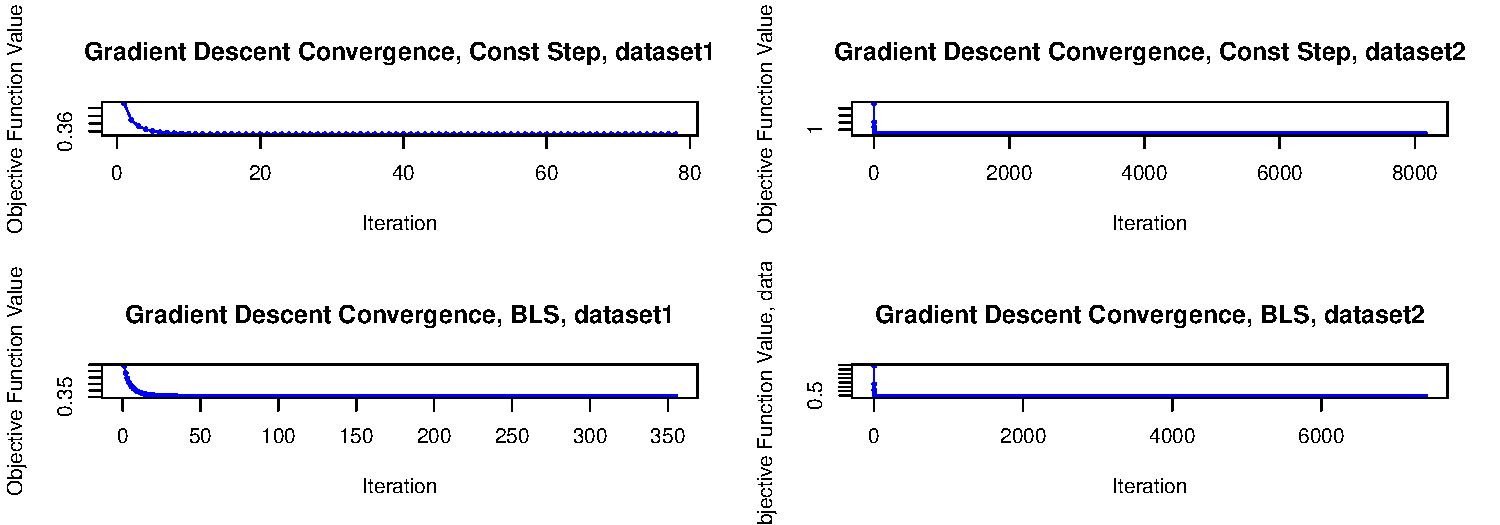
\includegraphics{506021334_Stats102B_hw_1_files/figure-pdf/2-a-3-1.pdf}

\subsection{Part b}\label{part-b-1}

\textbf{Implement the Polyak and Nesterov momentum methods and obtain
the estimates of the regression coefficients, using both a constant step
size and backtracking line search}




\end{document}
